% Options for packages loaded elsewhere
\PassOptionsToPackage{unicode}{hyperref}
\PassOptionsToPackage{hyphens}{url}
%
\documentclass[
]{book}
\usepackage{lmodern}
\usepackage{amssymb,amsmath}
\usepackage{ifxetex,ifluatex}
\ifnum 0\ifxetex 1\fi\ifluatex 1\fi=0 % if pdftex
  \usepackage[T1]{fontenc}
  \usepackage[utf8]{inputenc}
  \usepackage{textcomp} % provide euro and other symbols
\else % if luatex or xetex
  \usepackage{unicode-math}
  \defaultfontfeatures{Scale=MatchLowercase}
  \defaultfontfeatures[\rmfamily]{Ligatures=TeX,Scale=1}
\fi
% Use upquote if available, for straight quotes in verbatim environments
\IfFileExists{upquote.sty}{\usepackage{upquote}}{}
\IfFileExists{microtype.sty}{% use microtype if available
  \usepackage[]{microtype}
  \UseMicrotypeSet[protrusion]{basicmath} % disable protrusion for tt fonts
}{}
\makeatletter
\@ifundefined{KOMAClassName}{% if non-KOMA class
  \IfFileExists{parskip.sty}{%
    \usepackage{parskip}
  }{% else
    \setlength{\parindent}{0pt}
    \setlength{\parskip}{6pt plus 2pt minus 1pt}}
}{% if KOMA class
  \KOMAoptions{parskip=half}}
\makeatother
\usepackage{xcolor}
\IfFileExists{xurl.sty}{\usepackage{xurl}}{} % add URL line breaks if available
\IfFileExists{bookmark.sty}{\usepackage{bookmark}}{\usepackage{hyperref}}
\hypersetup{
  pdftitle={Materials for ECON200: Introductory Macroeconomics},
  pdfauthor={Andre R. Neveu},
  hidelinks,
  pdfcreator={LaTeX via pandoc}}
\urlstyle{same} % disable monospaced font for URLs
\usepackage{longtable,booktabs}
% Correct order of tables after \paragraph or \subparagraph
\usepackage{etoolbox}
\makeatletter
\patchcmd\longtable{\par}{\if@noskipsec\mbox{}\fi\par}{}{}
\makeatother
% Allow footnotes in longtable head/foot
\IfFileExists{footnotehyper.sty}{\usepackage{footnotehyper}}{\usepackage{footnote}}
\makesavenoteenv{longtable}
\usepackage{graphicx,grffile}
\makeatletter
\def\maxwidth{\ifdim\Gin@nat@width>\linewidth\linewidth\else\Gin@nat@width\fi}
\def\maxheight{\ifdim\Gin@nat@height>\textheight\textheight\else\Gin@nat@height\fi}
\makeatother
% Scale images if necessary, so that they will not overflow the page
% margins by default, and it is still possible to overwrite the defaults
% using explicit options in \includegraphics[width, height, ...]{}
\setkeys{Gin}{width=\maxwidth,height=\maxheight,keepaspectratio}
% Set default figure placement to htbp
\makeatletter
\def\fps@figure{htbp}
\makeatother
\setlength{\emergencystretch}{3em} % prevent overfull lines
\providecommand{\tightlist}{%
  \setlength{\itemsep}{0pt}\setlength{\parskip}{0pt}}
\setcounter{secnumdepth}{5}
\usepackage{booktabs}
\usepackage{longtable}
\usepackage{array}
\usepackage{multirow}
\usepackage{wrapfig}
\usepackage{float}
\usepackage{colortbl}
\usepackage{pdflscape}
\usepackage{tabu}
\usepackage{threeparttable}
\usepackage{threeparttablex}
\usepackage[normalem]{ulem}
\usepackage{makecell}
\usepackage{xcolor}
\usepackage{booktabs}
\usepackage{longtable}
\usepackage{array}
\usepackage{multirow}
\usepackage{wrapfig}
\usepackage{float}
\usepackage{colortbl}
\usepackage{pdflscape}
\usepackage{tabu}
\usepackage{threeparttable}
\usepackage{threeparttablex}
\usepackage[normalem]{ulem}
\usepackage{makecell}
\usepackage{xcolor}
\usepackage[]{natbib}
\bibliographystyle{aer}

\title{Materials for ECON200: Introductory Macroeconomics}
\author{Andre R. Neveu}
\date{2020-05-20}

\begin{document}
\maketitle

{
\setcounter{tocdepth}{1}
\tableofcontents
}
\hypertarget{preface}{%
\chapter*{Preface}\label{preface}}
\addcontentsline{toc}{chapter}{Preface}

This site will include supplemental material to our regular macroeconomics course readings. Mostly this will be used to show you how we can use publicly available data to create tables and figures to help us understand and analyze the economy. This material will accompany \citet{tw} which will be the primary book for the course. We will also be using \citet{core}, and the other materials compiled by CORE including \emph{Economy, Society, \& Public Policy} \citep{espp} and \emph{Doing Economics} \citep{doing} which act as useful comparisons to the more traditional material presented in \citet{tw}.

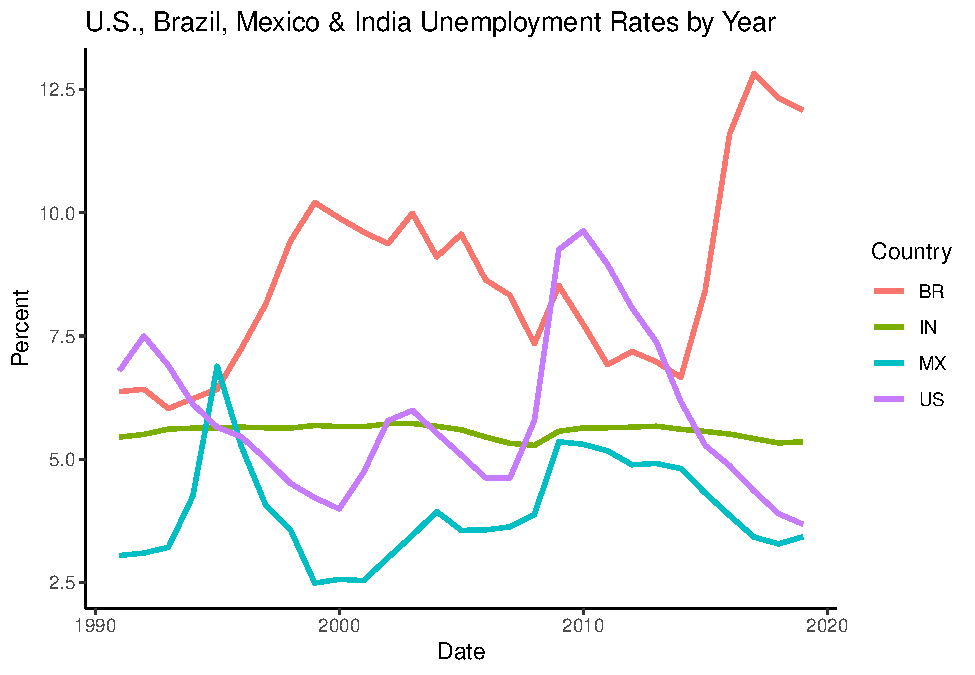
\includegraphics{econ200-book_files/figure-latex/unnamed-chunk-2-1.pdf}

\hypertarget{intro}{%
\chapter{Introduction}\label{intro}}

In Figure \ref{fig:unems} below, you will see the unemployment rate for four countries averaged over each year. The unemployment rate measures the percent of people who cannot find a job in the group of those people either working or looking for work. It seems like a mouthful, but we are estimating the proportion of people who are technically in the \emph{labor force}.

\begin{figure}

{\centering 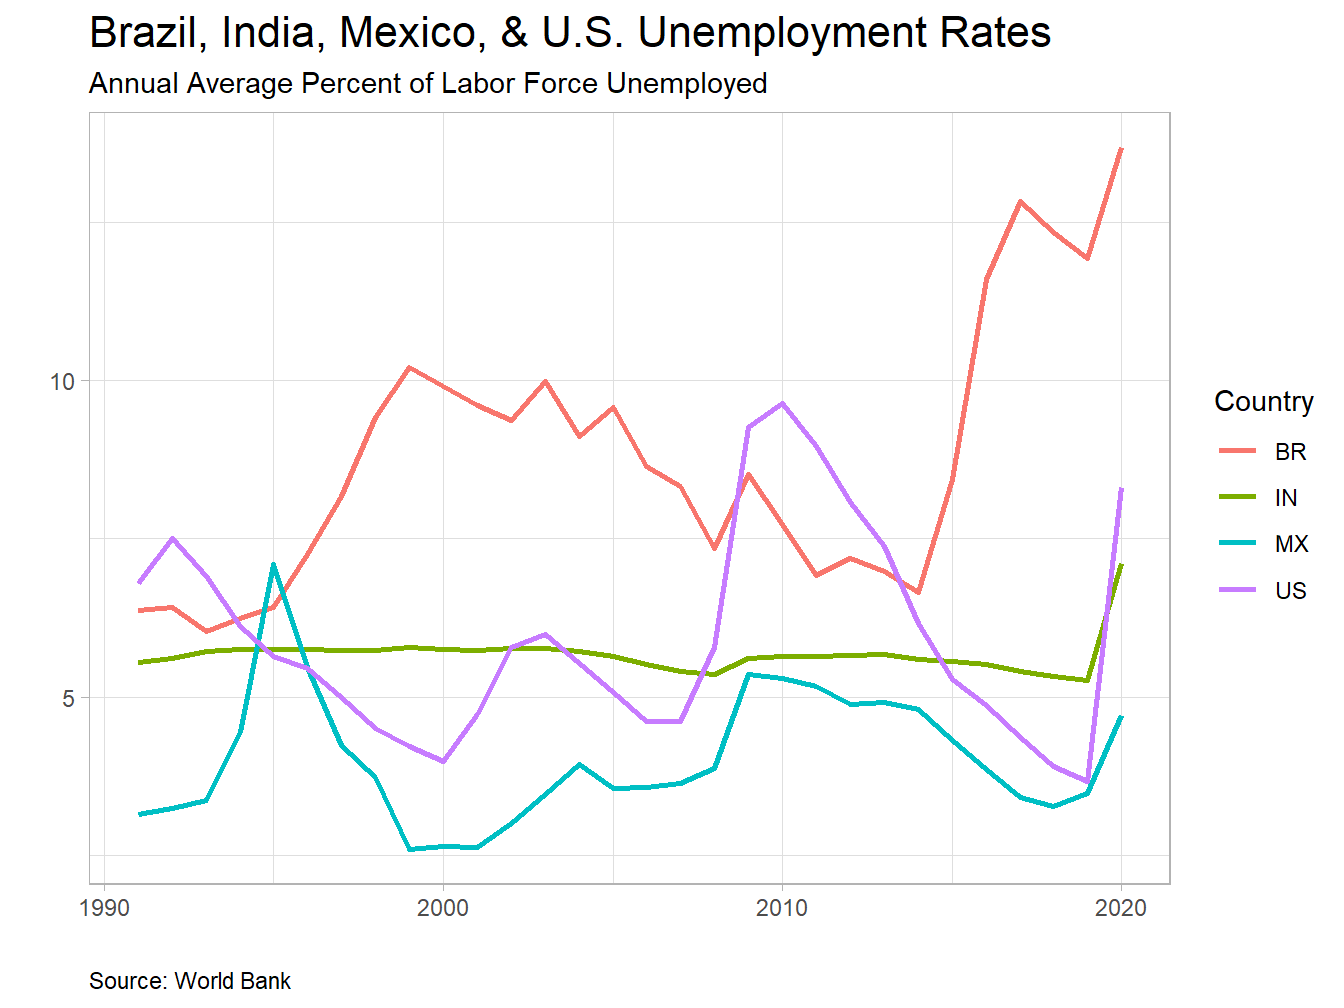
\includegraphics[width=0.8\linewidth]{econ200-book_files/figure-latex/unems-1} 

}

\caption{Unemployment Rates Around the World}\label{fig:unems}
\end{figure}

\begin{quote}
\textbf{Labor Force} is the sum of those who are employed and those actively looking for work.
\end{quote}

We measure the unemployment rate as:

\[ \text{Unemployment Rate} = \frac{\text{Unemployed}}{\text{Unemployed} + \text{Employed}} \times 100 \]

Something important about Figure \ref{fig:unems} is that we can see in some countries the unemployment rate is much higher than in other countries. Partially this is because we do not all use the same measurements for those who are either technically unemployed or working. However, if we assume countries do a consistent job in measuring these rates, the changes are still somewhat accurate. For example, in the United States a monthly survey of about 60,000 households counts those considered unemployed not just as those people collecting unemployment payments, but also includes all those people who have actively sought work in the past four weeks \href{https://www.bls.gov/cps/cps_htgm.htm}{(Bureau of Labor Statistics)}.

In recent months the COVID-19 crisis has gripped the world and put our global economy in a precarious position. As we can see from Figures \ref{fig:jobs} and \ref{fig:vmt} people who are newly jobless and travel in the U.S. have moved dramatically in opposite directions.

\begin{figure}

{\centering 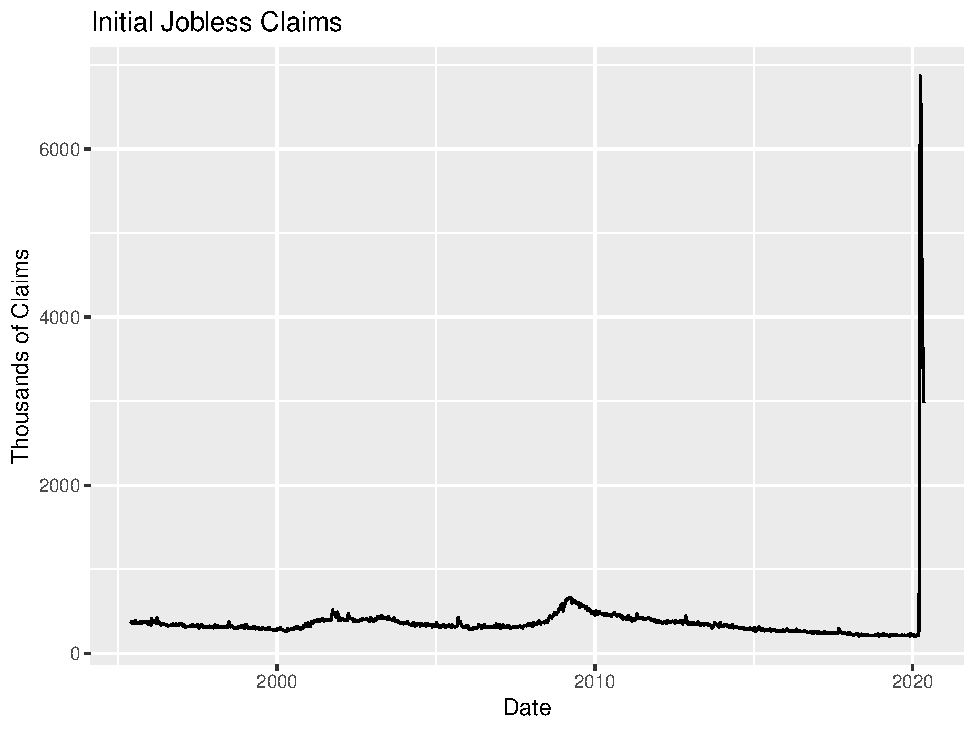
\includegraphics[width=0.8\linewidth]{econ200-book_files/figure-latex/jobs-1} 

}

\caption{Jobless Claims Skyrocket in 2020}\label{fig:jobs}
\end{figure}

\begin{figure}

{\centering 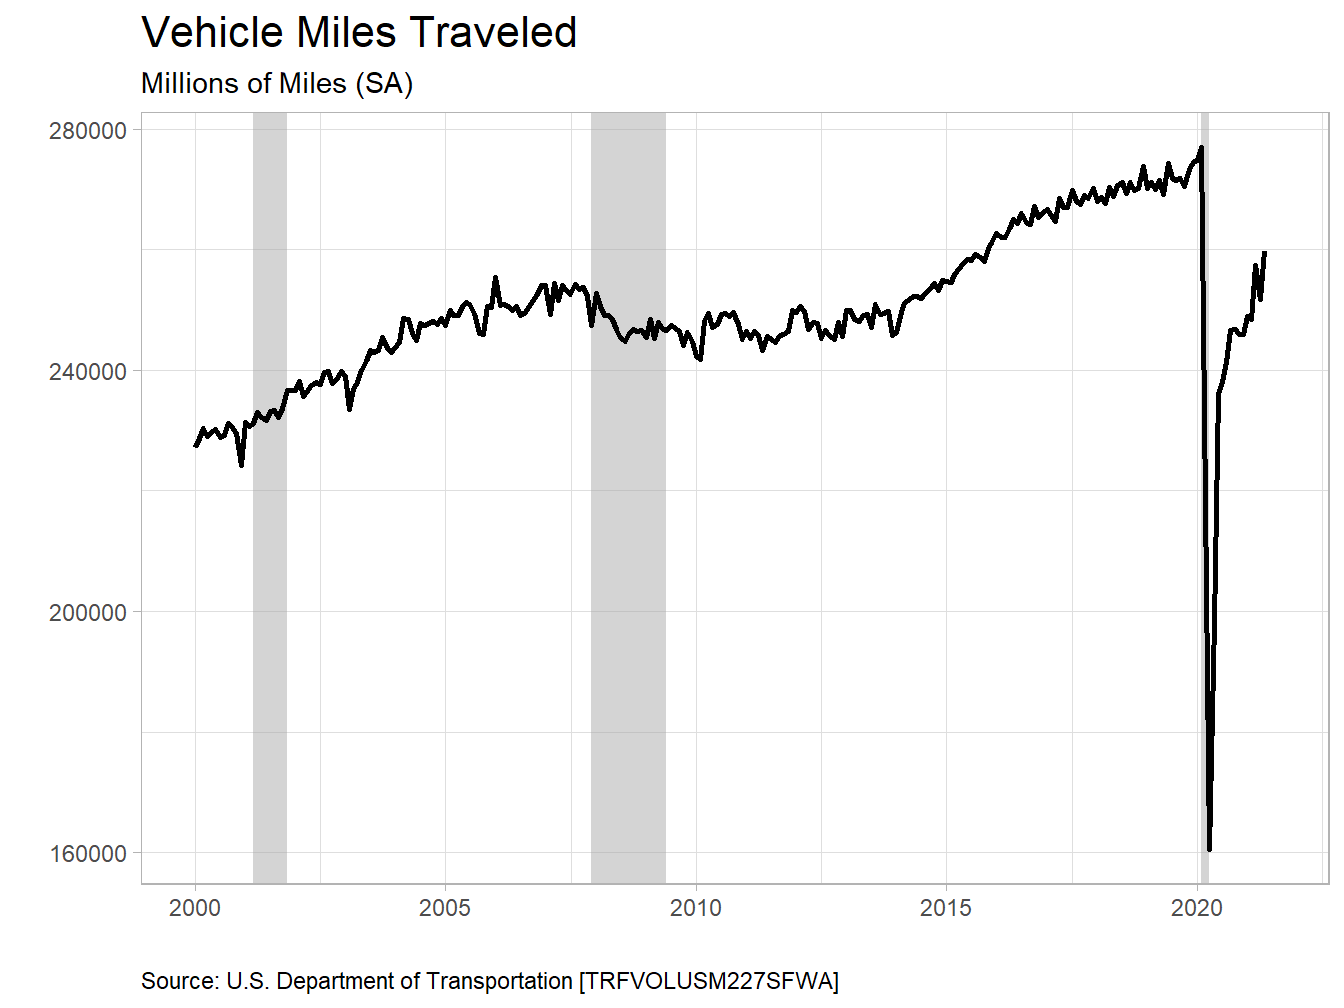
\includegraphics[width=0.8\linewidth]{econ200-book_files/figure-latex/vmt-1} 

}

\caption{Travel Collapses in 2020}\label{fig:vmt}
\end{figure}

Table \ref{tab:initial} shows the initial claims data for the past fifteen weeks, going back to the first weeks of the crisis in early March. Notice that the number of people filing for unemployment rose by a factor of more than ten! These unemployment claim numbers had literally never occurred in the U.S. before.

\begin{table}

\caption{\label{tab:initial}The Last 15 Weeks of Initial Unemployment Claims}
\centering
\begin{tabular}[t]{lr}
\toprule
Date & Claims\\
\midrule
2020-02-01 & 201000\\
2020-02-08 & 204000\\
2020-02-15 & 215000\\
2020-02-22 & 220000\\
2020-02-29 & 217000\\
\addlinespace
2020-03-07 & 211000\\
2020-03-14 & 282000\\
2020-03-21 & 3307000\\
2020-03-28 & 6867000\\
2020-04-04 & 6615000\\
\addlinespace
2020-04-11 & 5237000\\
2020-04-18 & 4442000\\
2020-04-25 & 3867000\\
2020-05-02 & 3176000\\
2020-05-09 & 2981000\\
\bottomrule
\end{tabular}
\end{table}

\hypertarget{money}{%
\chapter{Money Creation}\label{money}}

\hypertarget{money-debt-credit}{%
\section{Money, Debt, \& Credit}\label{money-debt-credit}}

Money is an abstract concept, closely linked to the notions of wealth, income, credit, and debt. While most people closely associate money with paper currency issued by governments, it is a much broader social and political construct. As a social construct, money functions as it does---facilitating exchange, measuring value, and storing value---because people agree that it exists. As a political construct, states authorize their money for the payment of taxes and require it to be accepted in payment for debts. In this sense, nations can be considered as the protectors of the debts between occupants of politically delineated boundaries. Money serves several functions. It is a medium of exchange; a unit of account; and a store of value. Money is also a standard of deferred payment.

As a medium of exchange, money is not the thing that is consumed in the process of trade but rather a symbol of agreed upon value. When a person sells their time to an employer, they are usually paid in money and not tangible consumption goods. The purpose of money in this instance is for the worker to ultimately use it in the future for their own consumption. Thus, there is an implicit agreement upon the value of the goods being exchanged (e.g., labor for time). Money also serves as a unit of account; in that it is how value is measured. In this way, money serves as standard of measurement. Thus, value of objects or actions can be measured and compared to one another. This is much the same as measuring height, weight, or speed. To serve as a store of value, money must retain most of its value over time. If one knew that money had no value at some point in the future, there would be no reason to accept it for exchange today. The store of value represents in some ways the trust that we place in one another when exchanging real things with each other over time.\footnote{Real variables would include things that can be measured objectively, like hiring someone to mow my lawn. The labor it takes to mow the lawn is real, as is the machine (i.e., physical capital) used to cut the lawn. The amount of a given currency paid to the worker or to buy the mower is a nominal variable since it is just representing relative value.} Currency issuing nations mandate the terms of payment of taxes, as well as the repayment of debts between a state and its people. Money also serves as a standard of deferred payment. A deferred payment happens when the time of purchase occurs separately from the time of payment. Money serves as the standard with which we value these payments (or debts). Since money represents a standard in inter-temporal commitment (e.g., goods or services are consumed today, but paid for next year), it serves as the object through which our debts and credits are settled with a state or in private transaction.

Money can be used to measure both stock and flow variables. Stock variables---like wealth---are measured at a given point in time. Below, balance sheets represent a typical way of measuring wealth (i.e., net worth) for individuals or capital (i.e., net equity) for companies. Flow variables---like income---are measured over a set length of time. Income might be paid as \$1,000 per week, or \$50,000 per year. Cash flow or income statements are common ways of measuring flow variables.

Debt is a stock concept, representing the sum of obligations owed to others at a given point in time. For example, you might have \$1,200 in accumulated debt at one point in time. Deficits or surpluses are flow concepts represented as the difference between income and expenditures over a set length of time. If you have \$500 a week in income, and \$600 in expenses, the result is a \$100 per-week deficit. In this example, after one week, debt would rise from \$1,200 to \$1,300 as the \$100 deficit is realized. Debts are the accumulated sum of all previous deficits and surpluses. It should be noted that debts do not need to be denominated in terms of an official state-issued currency. You could be in debt to a friend to ``give a ride'', ``move a couch'' or ``buy a drink'' without resorting to dollars or contracts. However, in the U.S., debt is generally measured in dollars. Debt is often inappropriately vilified, when the true concern might be that a person or entity has taken on too much debt. It might be better to think of debts as symbolizing promises of future real activity. It is common that some person or entity takes on more future real obligations than they might be able to deliver. In this case, when the time comes to collect on an earlier promise which cannot be fulfilled, both the debtor and creditor might renegotiate the terms of repayment.\footnote{Social and political norms can help arbitrate the renegotiation under certain circumstances like death. Suppose a person owes their bank \$1,000, but passes away suddenly. The bank might try to recoup their losses by taking over ownership of the person's house or car.} In most circumstances, debts are repaid. In this way, debt represents the social and community ties that take place over time. It is worth noting that whenever there is a delay in completing a transaction, debts are created. It is nearly impossible to think of a world in which debt does not exist or one where it is outlawed. Hence, debt and money represent a special kind of social contract.

As is explained below, people and banks can create money out of thin air. Today, when an obligation which spans time is entered into between two parties, this debt is measured using money. In this way, a \$10 bill represents future real activity that someone will do for you. Cash, somewhat counterintuitively, is a symbol of debt. If you read a U.S. Federal Reserve Note (U.S. paper money) it says on the front, that ``This note is legal tender for all debts, public and private.'' To the person holding physical or electronic cash, it means either you can repay your debts with it, or you can unlock real activity from someone else by getting them to do something for you. A wealthy individual---like Mark Zuckerberg---holds a great deal of influence over what other people will be doing in the future.

\hypertarget{wealth-and-balance-sheets}{%
\section{Wealth and Balance Sheets}\label{wealth-and-balance-sheets}}

With the concepts of money, debt, and credit introduced, an example can be developed. Imagine that Logan owns several assets. Let's say he has \$1,000 in a checking account, \$60 in cash, a computer he values at \$800, a phone valued at \$500, and a bike worth \$300. These values are what he thinks he can sell these to someone else for. We measure the object's liquidity as the speed you can turn an asset into cash, without significant loss in value. Cash and deposits are generally the most liquid assets, since there is minimal risk that it is not worth exactly what you think it is (e.g., \$100 can be sold for \$100). However, a computer, phone, or bike might not sell right away (or ever) at the values you estimate.

We then examine Logan's liabilities, or obligations to others. If he owes \$1,000 to his credit card company, and has \$3,000 in student loans, he has promised to repay those amounts---likely with interest---at some point in the future. We define wealth as the difference between your total asset value and total liabilities. This difference is called wealth or net worth for individuals and capital or net equity for firms and banks. A balance sheet equates total asset value (usually shown on the left-hand side) with total liabilities plus net worth (usually both shown on the right-hand side).

\[ \text{Assets}=\text{Liabilities}+\text{Net Worth}\]

Using these values for the things Logan owns (\$2,660) and debts he owes to others (\$4,000), he would have a net worth of -\$1,340. We need to emphasize that net worth is the item on our balance sheet that balances the right-hand and left-hand side of Table \ref{tab:break}.

\begin{table}

\caption{\label{tab:break}Logan’s Household Balance Sheet}
\centering
\begin{tabular}[t]{>{\bfseries}lr|>{\bfseries}ll}
\toprule
Assets &  & Liabilities + Net Worth & \\
\midrule
Cash & 60 & Credit Card & 1000\\
Deposits & 1000 & Student Loan & 3000\\
Computer & 800 &  & \\
Phone & 500 &  & \\
Bike & 300 & Net Worth & -1340\\
\addlinespace
\rowcolor[HTML]{666666}  \textcolor{white}{\textbf{Total}} & \textcolor{white}{\textbf{2660}} & \textcolor{white}{\textbf{Total}} & \textcolor{white}{\textbf{2660}}\\
\bottomrule
\end{tabular}
\end{table}

\hypertarget{methods}{%
\chapter{Methods}\label{methods}}

We describe our methods in this chapter.

\hypertarget{applications}{%
\chapter{Applications}\label{applications}}

Some \emph{significant} applications are demonstrated in this chapter.

\hypertarget{example-one}{%
\section{Example one}\label{example-one}}

\hypertarget{example-two}{%
\section{Example two}\label{example-two}}

\hypertarget{final-words}{%
\chapter{Final Words}\label{final-words}}

We have finished a nice book.

  \bibliography{refs.bib}

\end{document}
